\section{genericRPG.h File Reference}
\label{genericRPG_8h}\index{genericRPG.h@{genericRPG.h}}
{\tt \#include \char`\"{}../../randomNumbers/impl/libRandom.hpp\char`\"{}}\par
{\tt \#include \char`\"{}../interfaces/processor.h\char`\"{}}\par
{\tt \#include \char`\"{}genericInterface.h\char`\"{}}\par
{\tt \#include \char`\"{}genericData.h\char`\"{}}\par
{\tt \#include $<$fstream$>$}\par
{\tt \#include $<$deque$>$}\par


Include dependency graph for genericRPG.h:\nopagebreak
\begin{figure}[H]
\begin{center}
\leavevmode
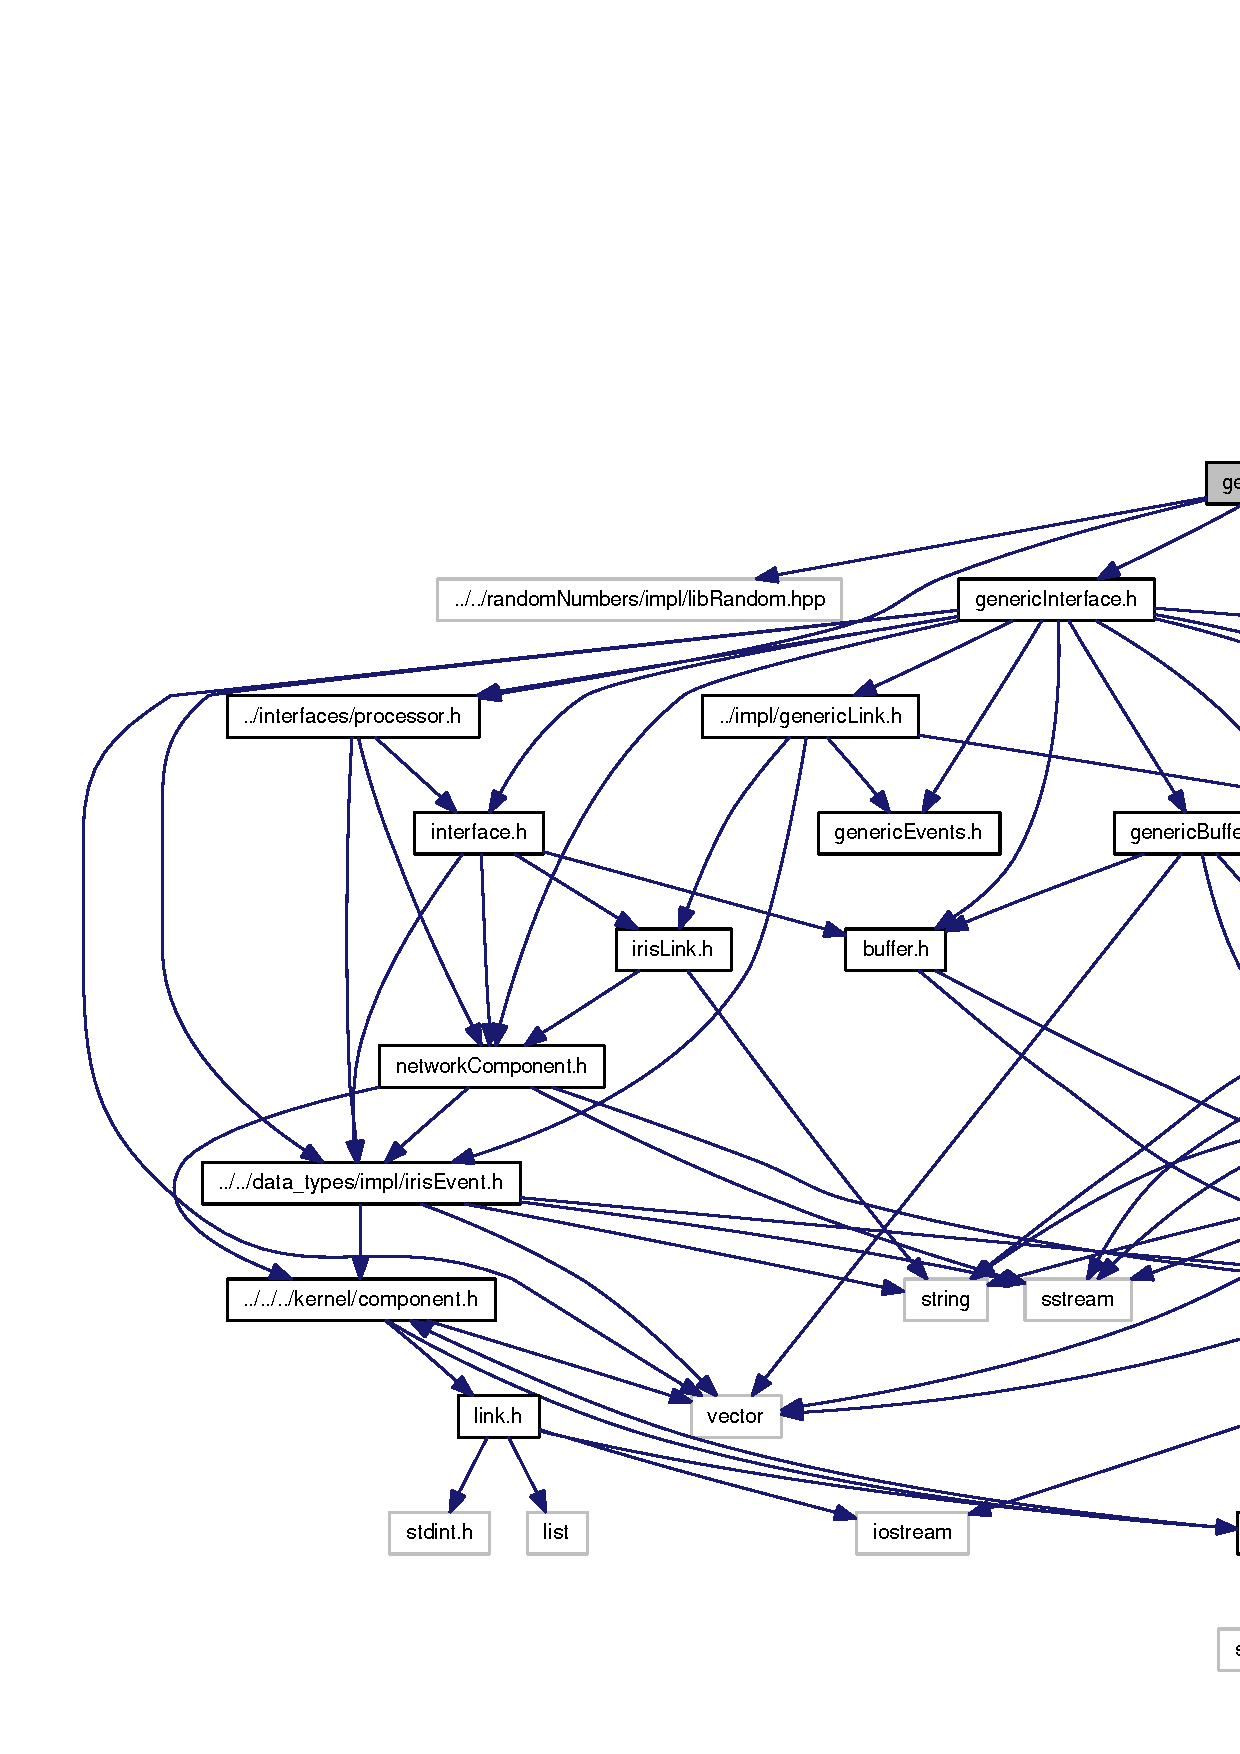
\includegraphics[width=420pt]{genericRPG_8h__incl}
\end{center}
\end{figure}


This graph shows which files directly or indirectly include this file:\nopagebreak
\begin{figure}[H]
\begin{center}
\leavevmode
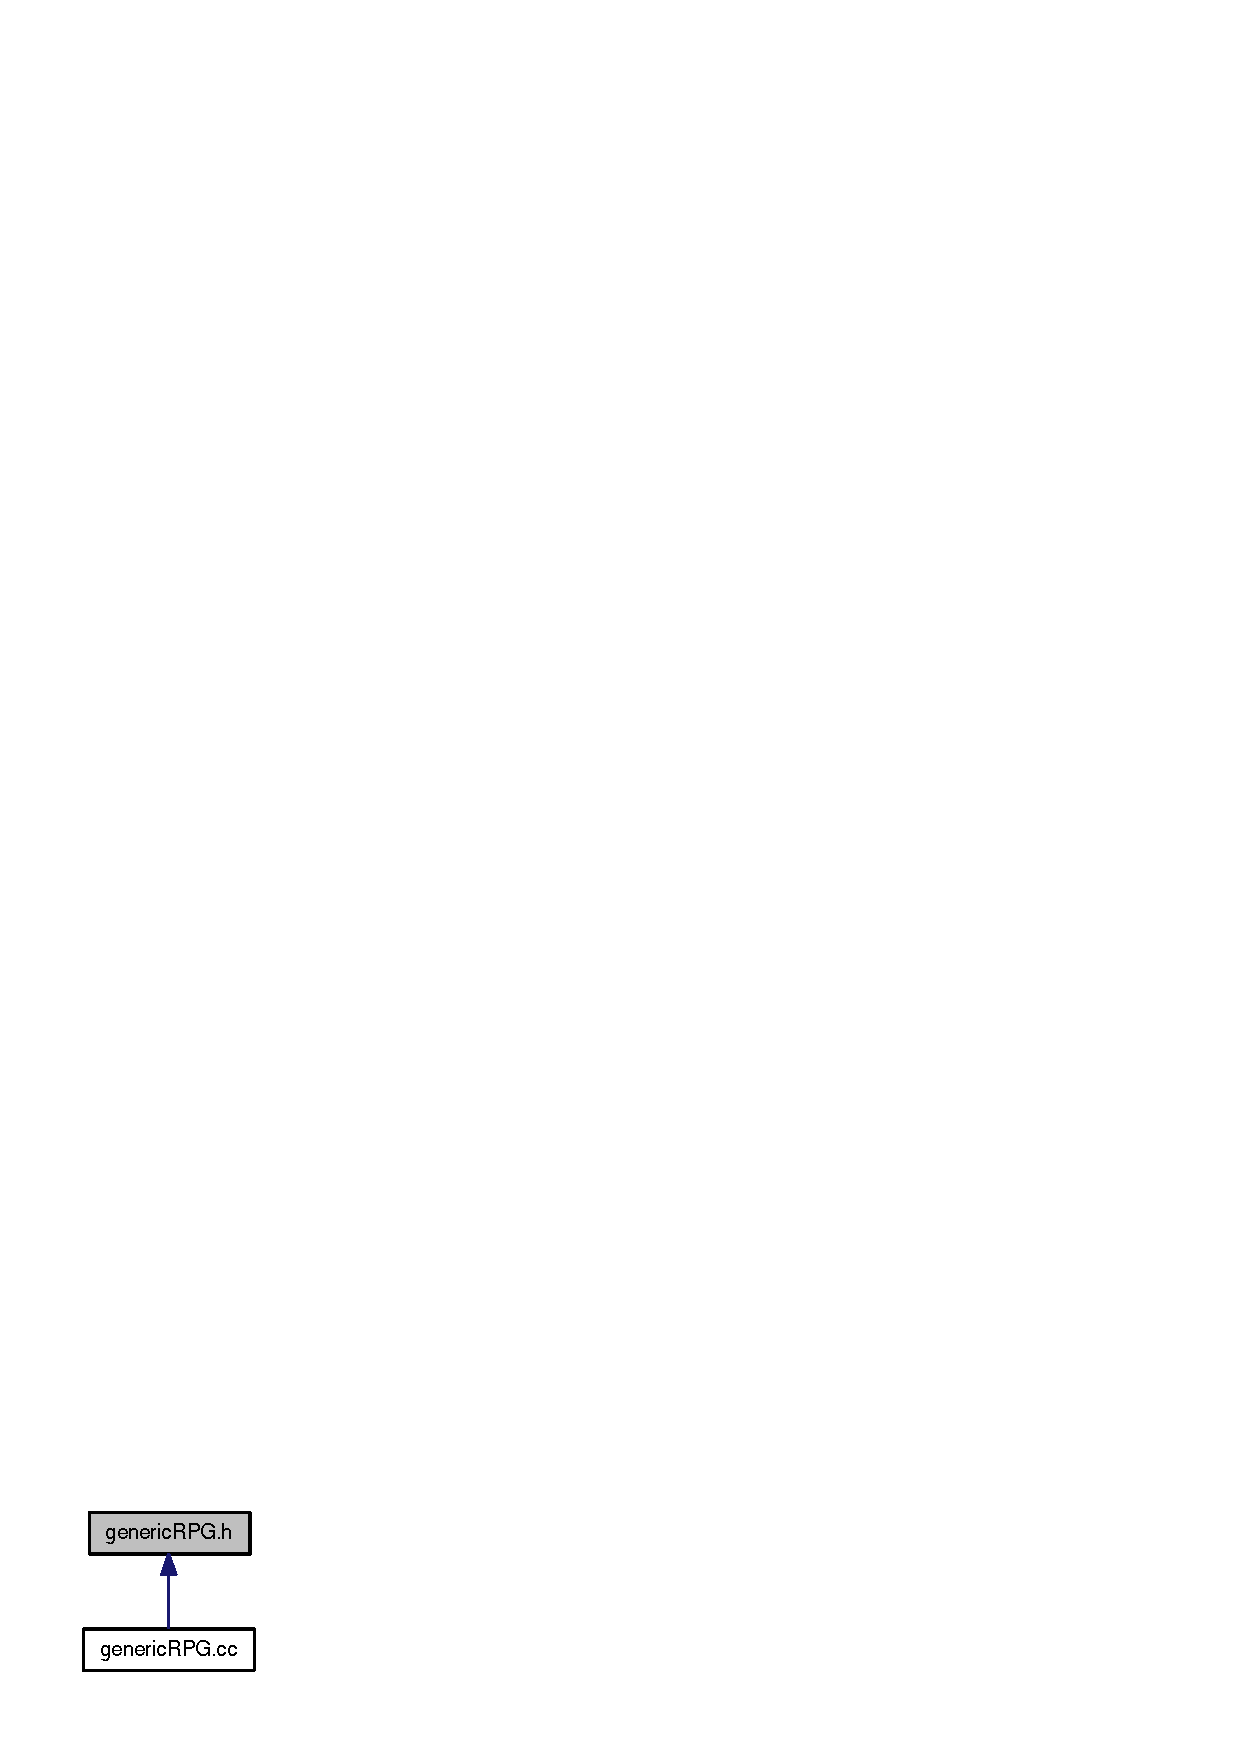
\includegraphics[width=63pt]{genericRPG_8h__dep__incl}
\end{center}
\end{figure}
\subsection*{Classes}
\begin{CompactItemize}
\item 
class {\bf GenericRPG}
\end{CompactItemize}
\subsection*{Defines}
\begin{CompactItemize}
\item 
\#define {\bf IN\_\-OUT\_\-MISMATCH}~-1
\item 
\#define {\bf SIM\_\-SUCCESS}~0
\item 
\#define {\bf REPORT\_\-BASE}~20
\item 
\#define {\bf DEFAULT\_\-RAN\_\-LAMDA}~2.35
\item 
\#define {\bf DEFAULT\_\-RAN\_\-DESTINATION\_\-TYPE}~\char`\"{}uniform\char`\"{}
\item 
\#define {\bf DEFAULT\_\-RAN\_\-LENGTH\_\-TYPE}~\char`\"{}uniform\char`\"{}
\item 
\#define {\bf DEFAULT\_\-RAN\_\-ADDRESS}~0
\item 
\#define {\bf MAX\_\-ADDRESS}~3
\item 
\#define {\bf MAX\_\-LENGTH}~10
\item 
\#define {\bf MIN\_\-LENGTH}~1
\item 
\#define {\bf MIN\_\-DELAY}~1
\item 
\#define {\bf MAX\_\-DELAY}~100
\item 
\#define {\bf DEFAULT\_\-RAN\_\-MAX\_\-VC}~1
\item 
\#define {\bf DEFAULT\_\-RAN\_\-SEED}~324986
\item 
\#define {\bf DEFAULT\_\-RAN\_\-MAX\_\-TIME}~100
\item 
\#define {\bf HOT\_\-SPOTS}~3
\item 
\#define {\bf DEFAULT\_\-RAN\_\-TRACE\_\-FILE\_\-NAME}~\char`\"{}randomOut.tr\char`\"{}
\item 
\#define {\bf MAX}(a, b)~(((a)$<$(b))?(b):(a))
\item 
\#define {\bf MIN}(a, b)~(((a)$<$(b))?(a):(b))
\end{CompactItemize}
\subsection*{Variables}
\begin{CompactItemize}
\item 
const string {\bf run\_\-destination\_\-type} = \char`\"{}uniform\char`\"{}
\end{CompactItemize}


\subsection{Define Documentation}
\index{genericRPG.h@{genericRPG.h}!DEFAULT\_\-RAN\_\-ADDRESS@{DEFAULT\_\-RAN\_\-ADDRESS}}
\index{DEFAULT\_\-RAN\_\-ADDRESS@{DEFAULT\_\-RAN\_\-ADDRESS}!genericRPG.h@{genericRPG.h}}
\subsubsection[{DEFAULT\_\-RAN\_\-ADDRESS}]{\setlength{\rightskip}{0pt plus 5cm}\#define DEFAULT\_\-RAN\_\-ADDRESS~0}\label{genericRPG_8h_d9ab56612febb84dbf32c4bc009d8e94}




Definition at line 30 of file genericRPG.h.\index{genericRPG.h@{genericRPG.h}!DEFAULT\_\-RAN\_\-DESTINATION\_\-TYPE@{DEFAULT\_\-RAN\_\-DESTINATION\_\-TYPE}}
\index{DEFAULT\_\-RAN\_\-DESTINATION\_\-TYPE@{DEFAULT\_\-RAN\_\-DESTINATION\_\-TYPE}!genericRPG.h@{genericRPG.h}}
\subsubsection[{DEFAULT\_\-RAN\_\-DESTINATION\_\-TYPE}]{\setlength{\rightskip}{0pt plus 5cm}\#define DEFAULT\_\-RAN\_\-DESTINATION\_\-TYPE~\char`\"{}uniform\char`\"{}}\label{genericRPG_8h_09f738f8baf435b6537768cc94dad17d}




Definition at line 28 of file genericRPG.h.\index{genericRPG.h@{genericRPG.h}!DEFAULT\_\-RAN\_\-LAMDA@{DEFAULT\_\-RAN\_\-LAMDA}}
\index{DEFAULT\_\-RAN\_\-LAMDA@{DEFAULT\_\-RAN\_\-LAMDA}!genericRPG.h@{genericRPG.h}}
\subsubsection[{DEFAULT\_\-RAN\_\-LAMDA}]{\setlength{\rightskip}{0pt plus 5cm}\#define DEFAULT\_\-RAN\_\-LAMDA~2.35}\label{genericRPG_8h_96e8def35c4a4089d135b84a42ba3ef5}




Definition at line 27 of file genericRPG.h.\index{genericRPG.h@{genericRPG.h}!DEFAULT\_\-RAN\_\-LENGTH\_\-TYPE@{DEFAULT\_\-RAN\_\-LENGTH\_\-TYPE}}
\index{DEFAULT\_\-RAN\_\-LENGTH\_\-TYPE@{DEFAULT\_\-RAN\_\-LENGTH\_\-TYPE}!genericRPG.h@{genericRPG.h}}
\subsubsection[{DEFAULT\_\-RAN\_\-LENGTH\_\-TYPE}]{\setlength{\rightskip}{0pt plus 5cm}\#define DEFAULT\_\-RAN\_\-LENGTH\_\-TYPE~\char`\"{}uniform\char`\"{}}\label{genericRPG_8h_800e5323ed643b94bc97133e37ea67b5}




Definition at line 29 of file genericRPG.h.\index{genericRPG.h@{genericRPG.h}!DEFAULT\_\-RAN\_\-MAX\_\-TIME@{DEFAULT\_\-RAN\_\-MAX\_\-TIME}}
\index{DEFAULT\_\-RAN\_\-MAX\_\-TIME@{DEFAULT\_\-RAN\_\-MAX\_\-TIME}!genericRPG.h@{genericRPG.h}}
\subsubsection[{DEFAULT\_\-RAN\_\-MAX\_\-TIME}]{\setlength{\rightskip}{0pt plus 5cm}\#define DEFAULT\_\-RAN\_\-MAX\_\-TIME~100}\label{genericRPG_8h_95a6218d50e244f6e58b6cca098c1d65}




Definition at line 38 of file genericRPG.h.\index{genericRPG.h@{genericRPG.h}!DEFAULT\_\-RAN\_\-MAX\_\-VC@{DEFAULT\_\-RAN\_\-MAX\_\-VC}}
\index{DEFAULT\_\-RAN\_\-MAX\_\-VC@{DEFAULT\_\-RAN\_\-MAX\_\-VC}!genericRPG.h@{genericRPG.h}}
\subsubsection[{DEFAULT\_\-RAN\_\-MAX\_\-VC}]{\setlength{\rightskip}{0pt plus 5cm}\#define DEFAULT\_\-RAN\_\-MAX\_\-VC~1}\label{genericRPG_8h_c317388cb88258db1d6de1ff7bcb1fda}




Definition at line 36 of file genericRPG.h.\index{genericRPG.h@{genericRPG.h}!DEFAULT\_\-RAN\_\-SEED@{DEFAULT\_\-RAN\_\-SEED}}
\index{DEFAULT\_\-RAN\_\-SEED@{DEFAULT\_\-RAN\_\-SEED}!genericRPG.h@{genericRPG.h}}
\subsubsection[{DEFAULT\_\-RAN\_\-SEED}]{\setlength{\rightskip}{0pt plus 5cm}\#define DEFAULT\_\-RAN\_\-SEED~324986}\label{genericRPG_8h_34af402b1c9a915b4114c54c6d7fa63c}




Definition at line 37 of file genericRPG.h.\index{genericRPG.h@{genericRPG.h}!DEFAULT\_\-RAN\_\-TRACE\_\-FILE\_\-NAME@{DEFAULT\_\-RAN\_\-TRACE\_\-FILE\_\-NAME}}
\index{DEFAULT\_\-RAN\_\-TRACE\_\-FILE\_\-NAME@{DEFAULT\_\-RAN\_\-TRACE\_\-FILE\_\-NAME}!genericRPG.h@{genericRPG.h}}
\subsubsection[{DEFAULT\_\-RAN\_\-TRACE\_\-FILE\_\-NAME}]{\setlength{\rightskip}{0pt plus 5cm}\#define DEFAULT\_\-RAN\_\-TRACE\_\-FILE\_\-NAME~\char`\"{}randomOut.tr\char`\"{}}\label{genericRPG_8h_8b605c4e6814dee663f4dcba1234f08f}




Definition at line 40 of file genericRPG.h.\index{genericRPG.h@{genericRPG.h}!HOT\_\-SPOTS@{HOT\_\-SPOTS}}
\index{HOT\_\-SPOTS@{HOT\_\-SPOTS}!genericRPG.h@{genericRPG.h}}
\subsubsection[{HOT\_\-SPOTS}]{\setlength{\rightskip}{0pt plus 5cm}\#define HOT\_\-SPOTS~3}\label{genericRPG_8h_416a5068ad5649b1fb0c4dc41d6616ff}




Definition at line 39 of file genericRPG.h.

Referenced by GenericRPG::init\_\-generator().\index{genericRPG.h@{genericRPG.h}!IN\_\-OUT\_\-MISMATCH@{IN\_\-OUT\_\-MISMATCH}}
\index{IN\_\-OUT\_\-MISMATCH@{IN\_\-OUT\_\-MISMATCH}!genericRPG.h@{genericRPG.h}}
\subsubsection[{IN\_\-OUT\_\-MISMATCH}]{\setlength{\rightskip}{0pt plus 5cm}\#define IN\_\-OUT\_\-MISMATCH~-1}\label{genericRPG_8h_acf2b8af3c21da41c625361742b49033}




Definition at line 14 of file genericRPG.h.\index{genericRPG.h@{genericRPG.h}!MAX@{MAX}}
\index{MAX@{MAX}!genericRPG.h@{genericRPG.h}}
\subsubsection[{MAX}]{\setlength{\rightskip}{0pt plus 5cm}\#define MAX(a, \/  b)~(((a)$<$(b))?(b):(a))}\label{genericRPG_8h_fa99ec4acc4ecb2dc3c2d05da15d0e3f}




Definition at line 42 of file genericRPG.h.

Referenced by sim\_\-print\_\-stats().\index{genericRPG.h@{genericRPG.h}!MAX\_\-ADDRESS@{MAX\_\-ADDRESS}}
\index{MAX\_\-ADDRESS@{MAX\_\-ADDRESS}!genericRPG.h@{genericRPG.h}}
\subsubsection[{MAX\_\-ADDRESS}]{\setlength{\rightskip}{0pt plus 5cm}\#define MAX\_\-ADDRESS~3}\label{genericRPG_8h_aba07841c3e227bc8bdd8ccdad149349}




Definition at line 31 of file genericRPG.h.\index{genericRPG.h@{genericRPG.h}!MAX\_\-DELAY@{MAX\_\-DELAY}}
\index{MAX\_\-DELAY@{MAX\_\-DELAY}!genericRPG.h@{genericRPG.h}}
\subsubsection[{MAX\_\-DELAY}]{\setlength{\rightskip}{0pt plus 5cm}\#define MAX\_\-DELAY~100}\label{genericRPG_8h_16027d8acc5301e440cefa086eb9db2a}




Definition at line 35 of file genericRPG.h.

Referenced by GenericRPG::init\_\-generator().\index{genericRPG.h@{genericRPG.h}!MAX\_\-LENGTH@{MAX\_\-LENGTH}}
\index{MAX\_\-LENGTH@{MAX\_\-LENGTH}!genericRPG.h@{genericRPG.h}}
\subsubsection[{MAX\_\-LENGTH}]{\setlength{\rightskip}{0pt plus 5cm}\#define MAX\_\-LENGTH~10}\label{genericRPG_8h_7a9a231e30b47bc0345749c8bd1e5077}




Definition at line 32 of file genericRPG.h.

Referenced by GenericRPG::init\_\-generator().\index{genericRPG.h@{genericRPG.h}!MIN@{MIN}}
\index{MIN@{MIN}!genericRPG.h@{genericRPG.h}}
\subsubsection[{MIN}]{\setlength{\rightskip}{0pt plus 5cm}\#define MIN(a, \/  b)~(((a)$<$(b))?(a):(b))}\label{genericRPG_8h_3acffbd305ee72dcd4593c0d8af64a4f}




Definition at line 43 of file genericRPG.h.\index{genericRPG.h@{genericRPG.h}!MIN\_\-DELAY@{MIN\_\-DELAY}}
\index{MIN\_\-DELAY@{MIN\_\-DELAY}!genericRPG.h@{genericRPG.h}}
\subsubsection[{MIN\_\-DELAY}]{\setlength{\rightskip}{0pt plus 5cm}\#define MIN\_\-DELAY~1}\label{genericRPG_8h_d3b51637a39a4ff75bd979b917cb89ef}




Definition at line 34 of file genericRPG.h.

Referenced by GenericRPG::init\_\-generator().\index{genericRPG.h@{genericRPG.h}!MIN\_\-LENGTH@{MIN\_\-LENGTH}}
\index{MIN\_\-LENGTH@{MIN\_\-LENGTH}!genericRPG.h@{genericRPG.h}}
\subsubsection[{MIN\_\-LENGTH}]{\setlength{\rightskip}{0pt plus 5cm}\#define MIN\_\-LENGTH~1}\label{genericRPG_8h_36aadcc60cb05b42dcda5459cd0c8acc}




Definition at line 33 of file genericRPG.h.

Referenced by GenericRPG::init\_\-generator().\index{genericRPG.h@{genericRPG.h}!REPORT\_\-BASE@{REPORT\_\-BASE}}
\index{REPORT\_\-BASE@{REPORT\_\-BASE}!genericRPG.h@{genericRPG.h}}
\subsubsection[{REPORT\_\-BASE}]{\setlength{\rightskip}{0pt plus 5cm}\#define REPORT\_\-BASE~20}\label{genericRPG_8h_acd7d711d1cb6daa442b1020836b7b10}




Definition at line 25 of file genericRPG.h.\index{genericRPG.h@{genericRPG.h}!SIM\_\-SUCCESS@{SIM\_\-SUCCESS}}
\index{SIM\_\-SUCCESS@{SIM\_\-SUCCESS}!genericRPG.h@{genericRPG.h}}
\subsubsection[{SIM\_\-SUCCESS}]{\setlength{\rightskip}{0pt plus 5cm}\#define SIM\_\-SUCCESS~0}\label{genericRPG_8h_7ff63f71612b54bc3472788c5cf858a8}




Definition at line 18 of file genericRPG.h.

\subsection{Variable Documentation}
\index{genericRPG.h@{genericRPG.h}!run\_\-destination\_\-type@{run\_\-destination\_\-type}}
\index{run\_\-destination\_\-type@{run\_\-destination\_\-type}!genericRPG.h@{genericRPG.h}}
\subsubsection[{run\_\-destination\_\-type}]{\setlength{\rightskip}{0pt plus 5cm}const string {\bf run\_\-destination\_\-type} = \char`\"{}uniform\char`\"{}}\label{genericRPG_8h_d2814df802952bf7d5e54b28efc5d6c5}




Definition at line 41 of file genericRPG.h.

Referenced by GenericRPG::setup().